\documentclass[12pt,oneside,letterpaper]{report}
\usepackage[spanish]{babel}
%\documentclass[a4paper,10pt]{scrartcl}

\usepackage[pdftex=true,colorlinks=,plainpages=false]{hyperref} % Soporte hipertexto

\usepackage[utf8x]{inputenc}
\usepackage{graphicx}

\title{Modelo de diseño}
\author{
Alejandro Palacio Duque\\
Sigifredo Escobar Gómez
}
\date{}

\pdfinfo{%
  /Title    (Modelo de diseño)
  /Author   (Sigifredo Escobar Gómez)
  /Creator  ()
  /Producer ()
  /Subject  ()
  /Keywords ()
}

\begin{document}

\maketitle

\tableofcontents	% Tabla de contenido
\listoffigures		% Índice de figuras

\newpage

\chapter{Descripción general del sistema}
\maketitle El sistema GyPI (Grupos y Proyectos de Investigación) gestionará los proyectos ya aceptados de los grupos de investigación permitiendo a las instancias administrativas de la Universidad de Antioquia centralizar la información de los diferentes grupos de investigación propiciando su acceso a la comunidad universitaria y al público en general.
El sistema permite registrar proyectos de investigación ya aprobados previamente, ingresando a cada uno de ellos los datos mas relevantes tales como (nombre, compromisos, cronograma, entre otros), de esta manera se logra tener un registro organizado y manejable sobre los proyectos que actualmente están siendo desarrollados en la Universidad. A demás de esto el sistema facilita a los  integrantes de un grupo de investigación le manejo de los compromisos y trámites tales como seguimiento a los compromisos necesarios para la culminación de un proyecto de investigación, solicitudes de prórrogas y cambios de investigador e informes sobre cambios relevantes en el proyecto al cual se encuentren vinculados .

\newpage

\chapter{Vistas}
\section{Vista de casos de uso}
\maketitle El sistema GyPI  ofrece los siguientes casos de uso:

% imagen
\begin{figure}[h!]
  \centering
    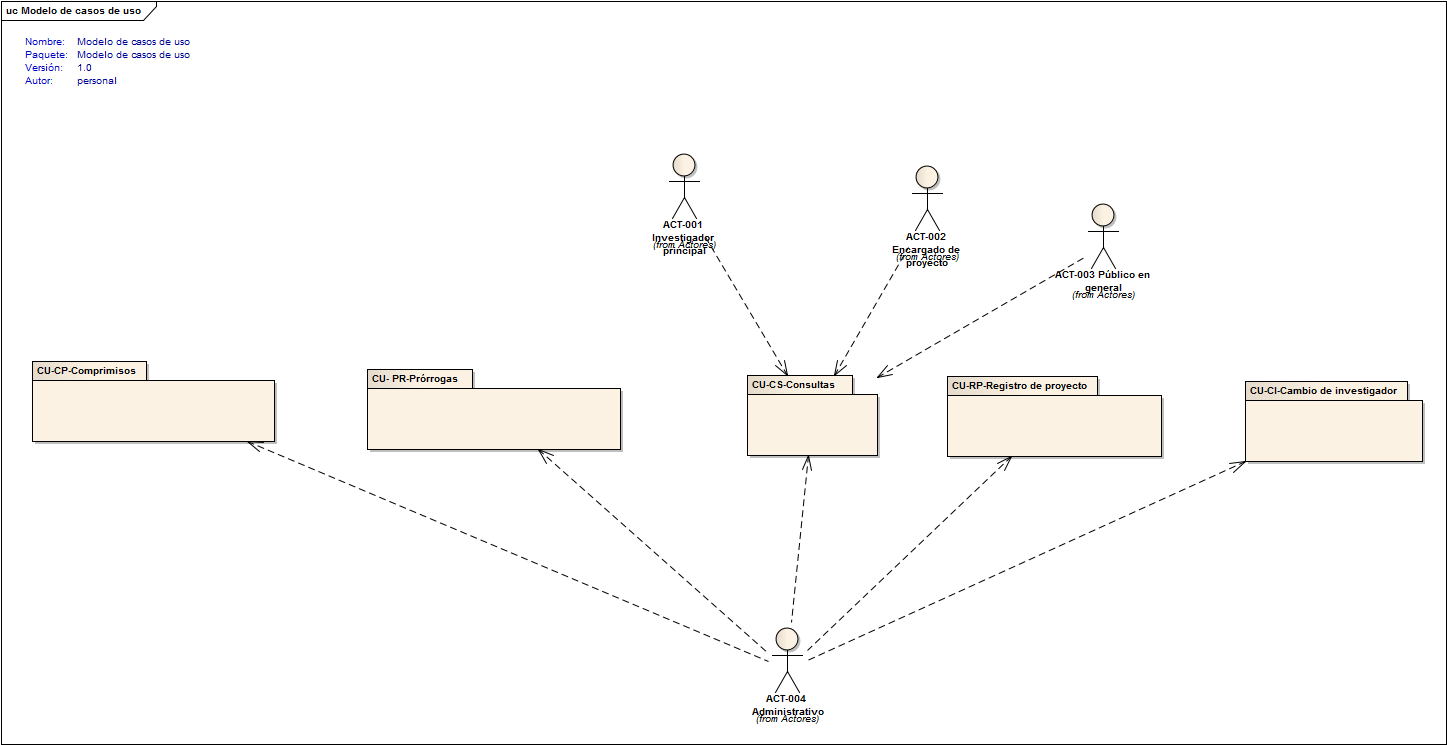
\includegraphics[width=0.75\textwidth]{./img/img1.png}
  \caption{Casos de uso}
\end{figure}

\maketitle A continuación se presentan cada uno de los casos de uso de manera mas detallada:

\textbf{CU-CS-Consultas:}
El sistema debe permitir realizar todo tipo de consultas sobre los grupos de investigación y sus respectivos proyectos. La información brindada en la consulta sera catalogada según el rol del usuario que la consulta de acuerdo con la regla de negocio RN-010 Acceso a la Información.

% imagen
\begin{figure}[h!]
  \centering
    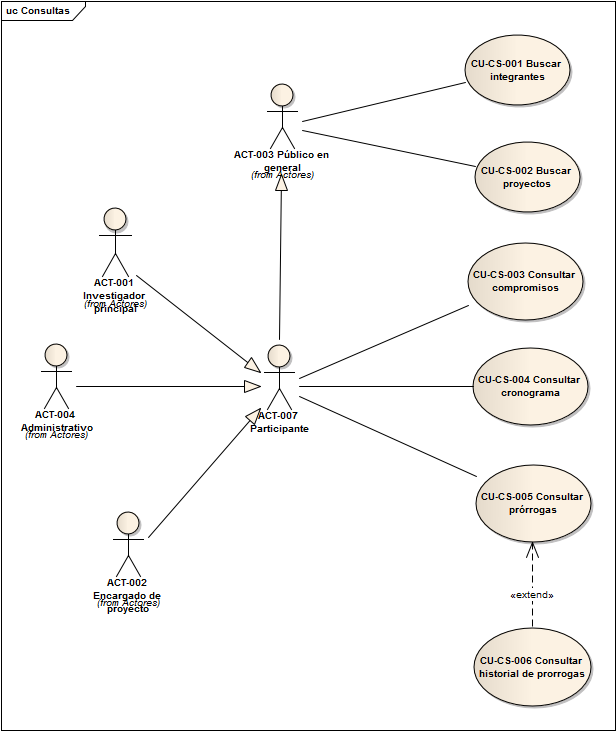
\includegraphics[width=0.75\textwidth]{./img/img2.png}
  \caption{Casos de uso de consultas}
\end{figure}

\textbf{CU-CI-Cambio de Investigador:}
El sistema debe permitir el registro de las solicitudes de cambio de investigador de un determinado proyecto. La solicitud para el cambio debe estar diligenciada de acuerdo a la regla de negocio RN-008 Cambio de Investigador.

% imagen
\begin{figure}[h!]
  \centering
    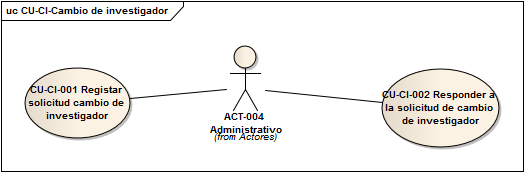
\includegraphics[width=0.75\textwidth]{./img/img3.png}
  \caption{Casos de uso de cambio de investigador}
\end{figure}

\textbf{CU-RP-Registro Proyecto:}
EL sistema debe permitir registrar un proyecto de investigación  de acuerdo con la regla de negocio RN-001 Registro de proyecto y sus respectivos componentes como lo son descripción (RN-003 Descripción de proyecto), investigador principal y responsable de proyecto  (RN-002 Investigador principal y responsable de proyecto), compromisos (RN-004 Compromisos), cronograma (RN-005 Cronograma), integrantes (RN-009 Validar usuario) e historial de prórrogas.

% imagen
\begin{figure}[h!]
  \centering
    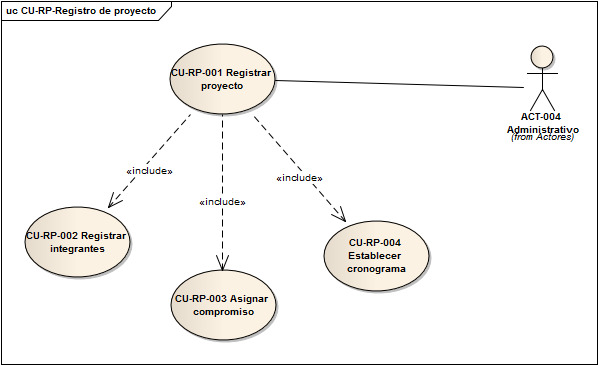
\includegraphics[width=0.75\textwidth]{./img/img4.png}
  \caption{Casos de uso de registro de proyecto}
\end{figure}

\textbf{CU-PR-Prórrogas}
El sistema debe permitir almacenar una solicitud de prórroga realizada por un grupo de investigación de acuerdo con las reglas de negocio  RN-006 prórrogas y RN-007 Solicitud de prórroga.

% imagen
\begin{figure}[h!]
  \centering
    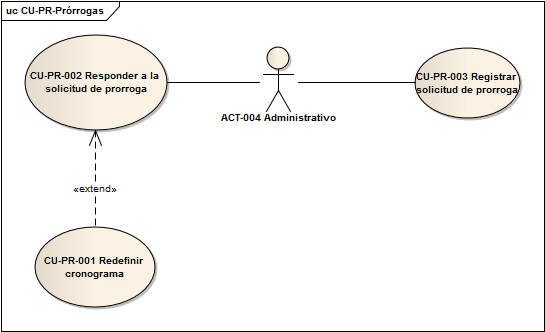
\includegraphics[width=0.75\textwidth]{./img/img5.png}
  \caption{Casos de uso de prórrogas}
\end{figure}

\textbf{CU-CP-Compromisos}

El sistema debe permitir realizar seguimiento a los compromisos de cada proyecto de investigación para tramitar y validar el cumplimiento o no de los mismos.

%imagen
\begin{figure}[h!]
  \centering
    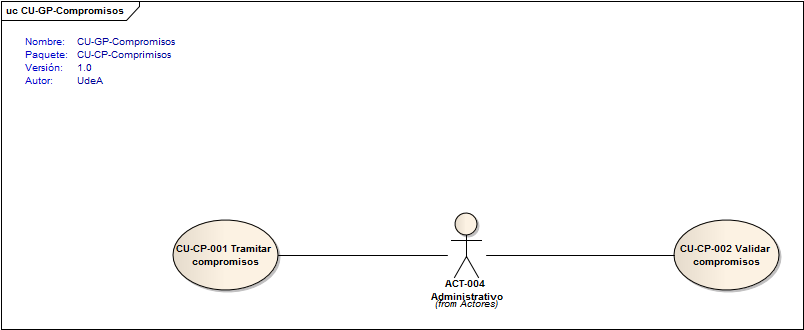
\includegraphics[width=0.75\textwidth]{./img/img6.png}
  \caption{Casos de uso de compromisos}
\end{figure}

\textbf{Requisitos de calidad}\\
\\
\textbf{QR-001 Consulta de información.} El sistema no deberá tardar mas de cinco segundos en dar respuesta a una bus queda de información por cualquiera de los usuarios que realice la consulta.\\
\\
\textbf{QR-002 Complejidad del sistema.} La aplicación deberá ser lo suficientemente sencilla para que el personal que se encargue de manejar la información comprenda de manera óptima el manejo de la misma.\\
\\
\textbf{QR-003 Parámetros de consulta.} El sistema de consultas deberá facilitar al máximo las búsquedas para los usuarios definiendo parámetros de búsqueda claros y legibles de manera que no se presenten ambigüedades en la búsqueda y el resultado sea mucho mas óptimo.\\
\\
\textbf{QR-004 Avisos del sistema.} El sistema deberá informar de manera oportuna sobre las fechas limites para responder a cada una de las solicitudes que se realicen a través del mismo.\\
\\
\textbf{QR-005 Accesibilidad.} El sistema deberá ser completamente accesible desde los principales navegadores web del mercado (firefox, chrome, Internet Explorer , Opera, Zafari).\\
\\
\textbf{QR-006 Seguridad de la información.} El sistema debe garantizar que la información va a permanecer segura y de manera persistente para su acceso.\\
\\
\textbf{QR-007 Almacenamiento de información.} El sistema debe contar con espacio en Disco suficientemente grande para garantizar el almacenamiento de los datos.\\
\\

\section{Vista de diseño}

\subsection{Diagrama de clases}

% imagen
\begin{figure}[h!]
  \centering
    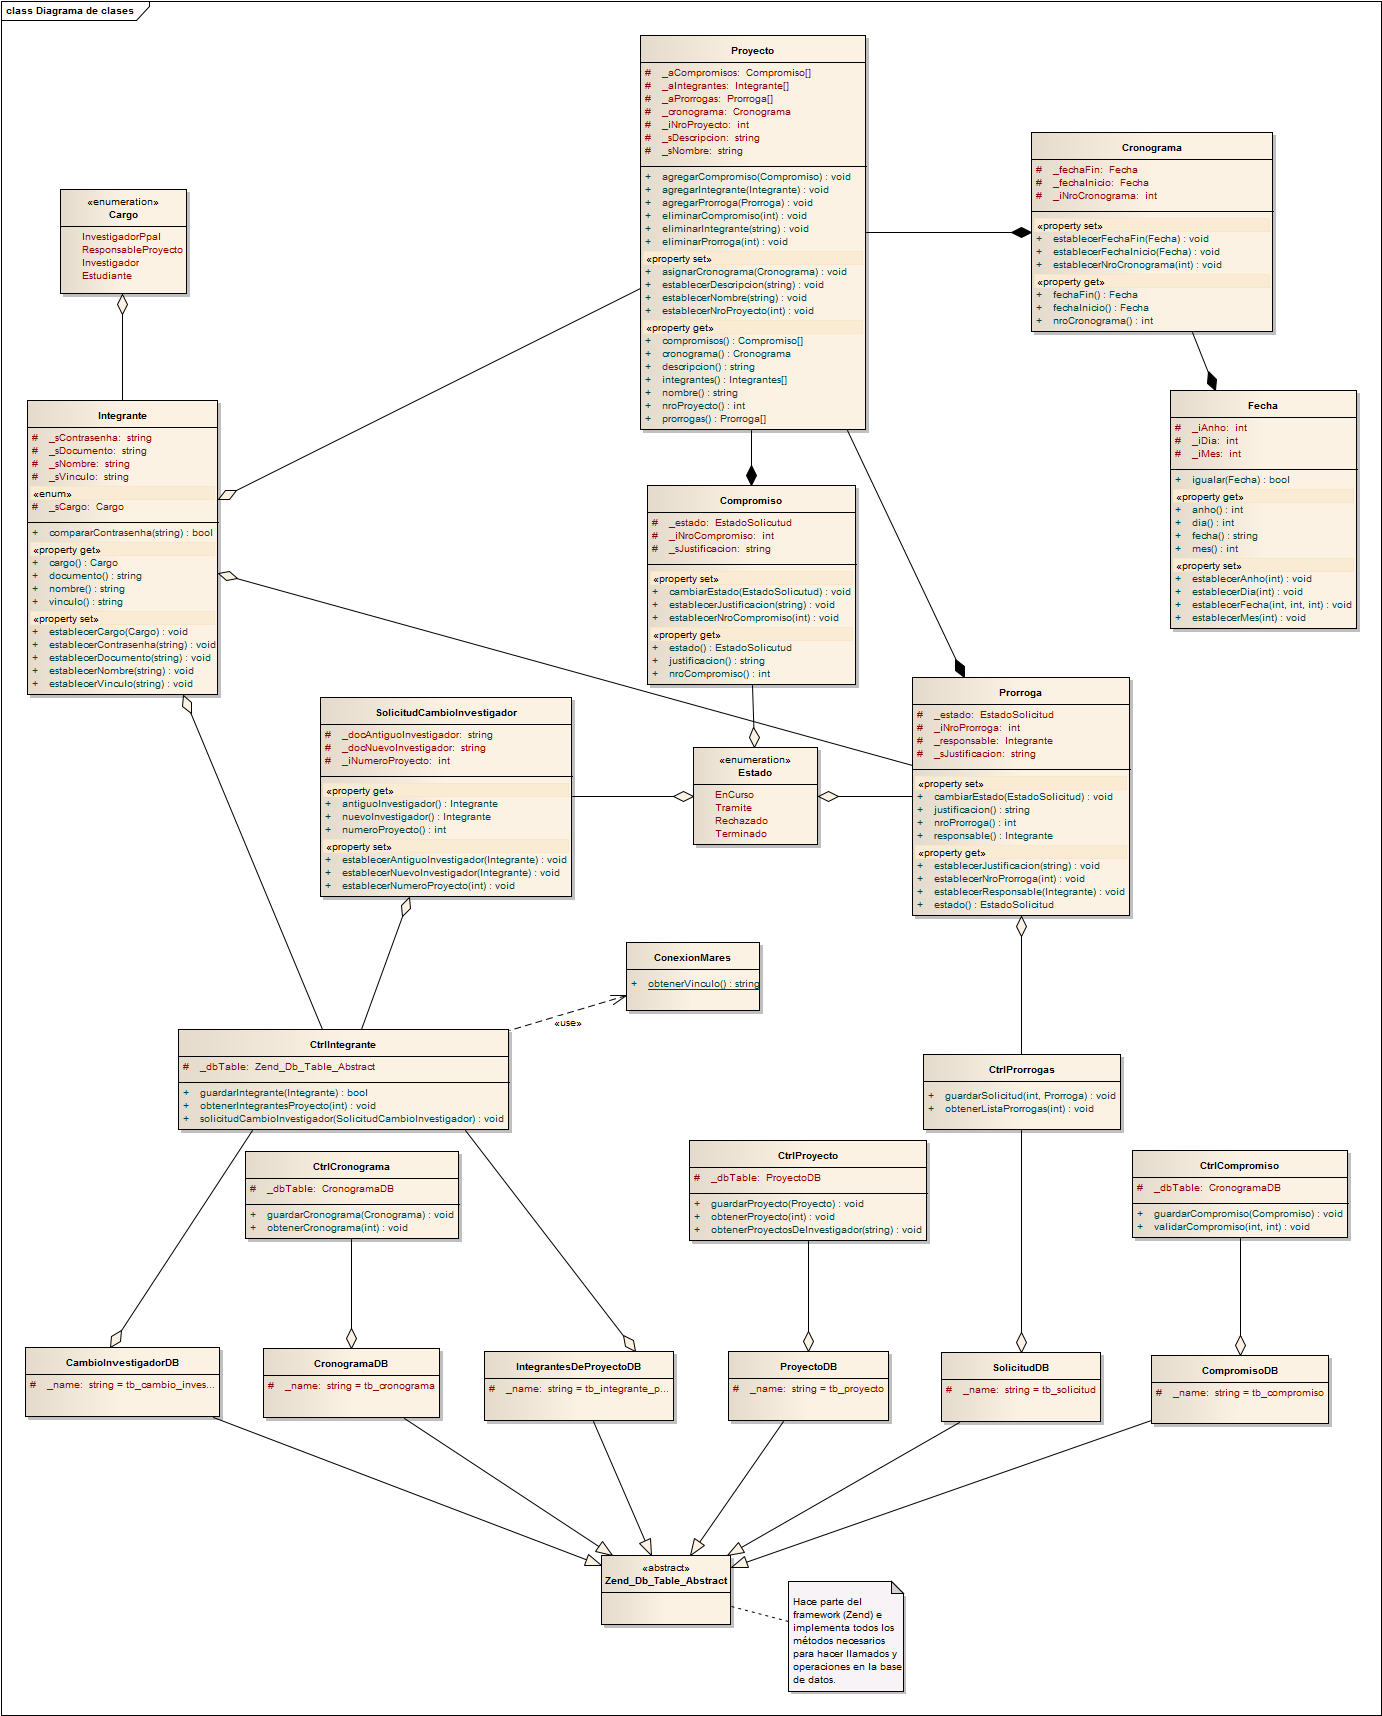
\includegraphics[width=0.75\textwidth]{./img/img7.png}
  \caption{Diagrama de clases}
\end{figure}


\textbf{Catalogo de elementos}\\

\begin{itemize}
 \item \textbf{Integrante:} se implementa una clase Integrante desarrollada en PHP la cual nos permite definir un integrante de un grupo de investigación.
 \item \textbf{FacadeConexionMares:} clase que implementa el patrón facade la cual nos representa el sistema Mares de la Universidad de Antioquia permitiendo así mediante esta obtener el vinculo que un integrante a registrar en un proyecto de investigación posee con la Universidad.
 \item \textbf{Proyecto:} se implementa una claseProyecto desarrollada en PHP que que representa un proyecto de investigación almacenado en el sistema.
 \item \textbf{Compromiso:} clase que define un compromiso vinculado a un proyecto.
 \item \textbf{prórroga:} clase desarrollada en PHP que representa una prórroga solicitada en un proyecto.
 \item \textbf{Cronograma:} clase desarrollada en PHP que define el cronograma estipulado para la culminación de un proyecto.
 \item \textbf{CtrlProyecto:} implementamos el patrón controller mediante la clase ctrlProyecto para que este se encargue de comunicarse con la interfaz que nos permite realizar operaciones sobre los proyectos registrados y este a su vez mediante sus métodos asigna a la clase proyecto la responsabilidad de ejecutar las acciones solicitadas por el usuario mediante la interfaz.
 \item \textbf{\textit{enumeration} Cargo:} clase que nos permite definir conjuntos de constantes enteras, llamados datos de tipo enumerado. Las variables declaradas de este tipo sólo podrán tomar valores dentro del dominio definido en la declaración en nuestro caso los cargos que puede tomar un integrante de un proyecto.
 \item \textbf{\textit{enumeration} Estado:} clase que implementa el estándar <<enumeration>> que nos permite seleccionar los estados que puede tener un proyecto de investigación.
 \item \textbf{Fecha:} clase que representa la fecha de inicio y final de algunas de las actividades del sistema que requieran de estas.
 \item \textbf{CambioInvestigadorDB:} clase que permite acceder a la base de datos para las operaciones pertinentes a un cambio de investigador.
 \item \textbf{CompromisoDB:} clase que permite acceder a la base de datos para las operaciones pertinentes a un compromiso.
 \item \textbf{CronogramaDB:} clase que permite acceder a la base de datos para las operaciones pertinentes a un cronograma.
 \item \textbf{ProyectoDB:} clase que permite acceder a la base de datos para las operaciones pertinentes a un proyecto.
 \item \textbf{ProrrogaDB:} clase que permite acceder a la base de datos para las operaciones pertinentes a una prorroga.
 \item \textbf{Zend\_Db\_Table\_Abstract:} clase que hace parte del framework (Zend) e implementa todos los métodos necesarios para hacer llamados y operaciones en la base de datos. Esta clase implementa el patrón singleton para tener una sola conexión a la base de datos y no consumir recursos estableciendo una conexión cada vez que se necesite interactuar con esta.
\end{itemize}


\textbf{Variabilidad:}
Mediante el archivo application.ini del framework ZEND se pueden cambiar los parámetros de conexión a la base de datos del sistema.\\

\textbf{Razón del diseño:}
El diseño del diagrama de clases fue basado en la aplicación de los patrones  de diseño GOF y GRASP los cuales nos facilitan la codificación y la asignación de responsabilidades en nuestro código. La aplicación de estos patrones se hace buscando que el sistema desarrollado tenga un bajo acoplamiento y una alta cohesión facilitando así la mantenibilidad de nuestro código y la reutilización del mismo.
El patrón facade se utiliza para proporcionar una interfaz unificada que nos permita comunicarnos con un subsistema en este caso Mares,simplificando el acceso a las clases de dicho sistema, ya que el cliente sólo se comunica con ellas a través de una única interfaz.\\

\textbf{Vistas relacionadas}
\begin{itemize}
\item Vista de procesos --- Diagrama de secuencias
\item Vista de implementación --- Diagrama de componentes
\item Vista de diseño --- Diagrama de objetos
\item Vista de diseño --- Diagrama de entidad – relación.
\item Vista de diseño --- Diagrama de entidad – relación.
\end{itemize}


\subsection{Diagrama Entidad - Relación}

% imagen
\begin{figure}[h!]
  \centering
    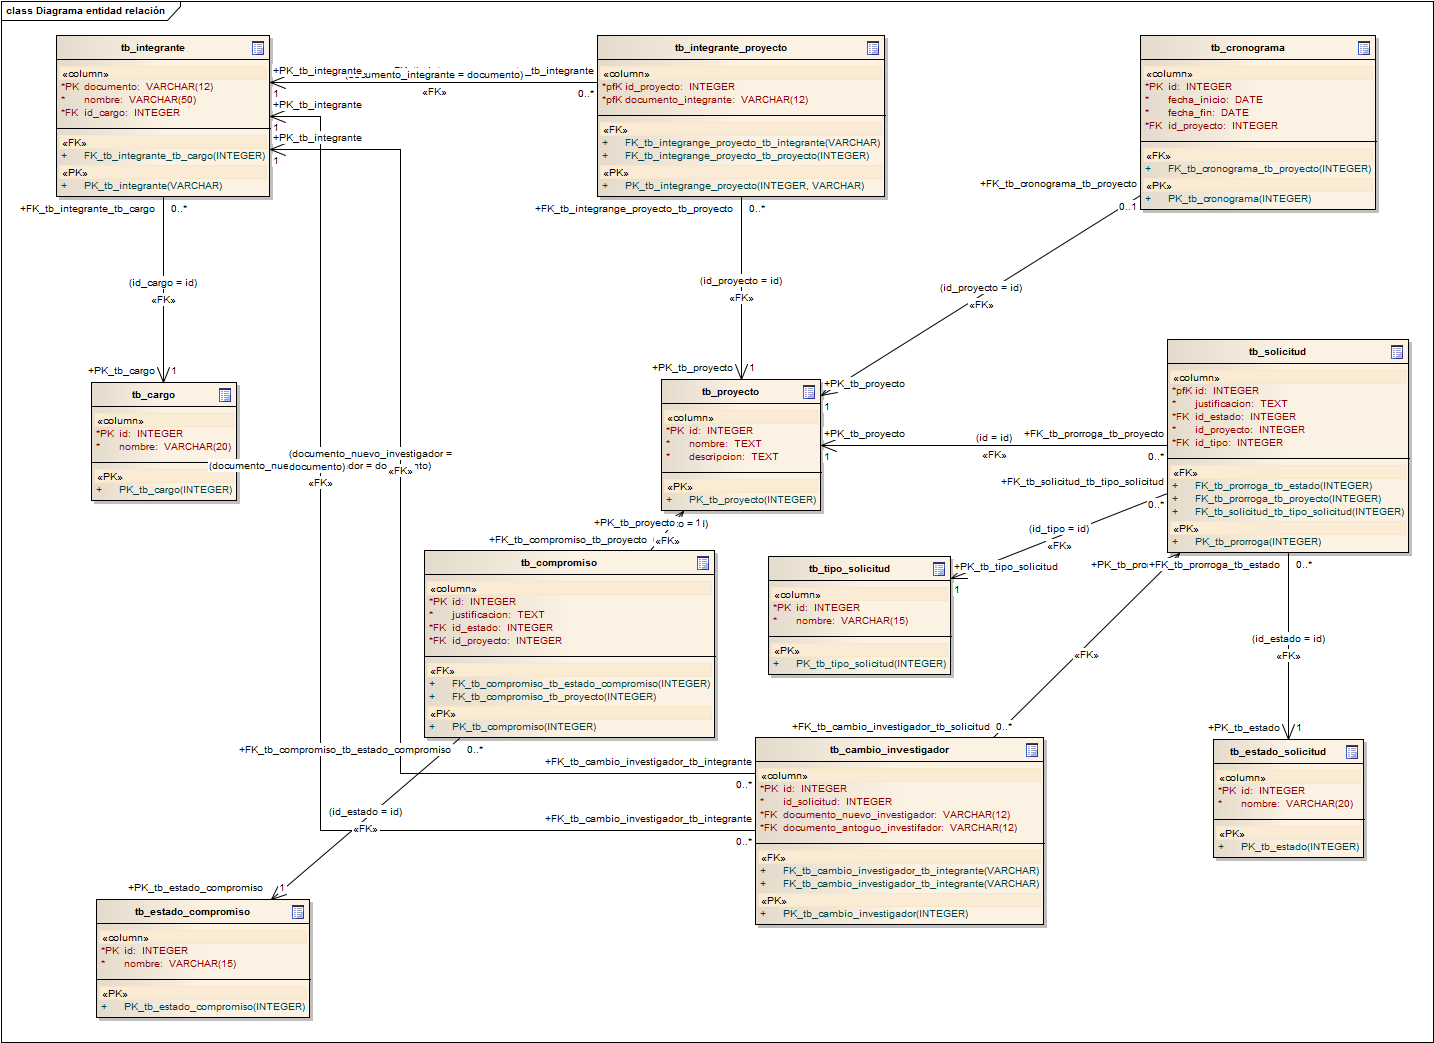
\includegraphics[width=0.75\textwidth]{./img/img8.png}
  \caption{Diagrama entidad relación}
\end{figure}


\textbf{Catalogo de elementos}\\

\begin{itemize}
 \item \textbf{tb\_integrante:} Esta tabla contiene los integrantes registrados en cada uno de los proyectos almacenados en el sistema.
 \item \textbf{tb\_cargo:} Esta tabla contiene los cargos que puede tener un integrante.
 \item \textbf{tb\_integrante\_proyecto:} Esta tabla relaciona cada integrante con su respectivo proyecto.
 \item \textbf{tb\_proyecto:} Esta tabla contiene los proyectos registrados en el sistema identificados cada uno por un numero único de registro.
 \item \textbf{tb\_compromiso:} Esta tabla contiene cada uno de los compromisos que tiene un proyecto.
 \item \textbf{tb\_estado\_compromiso:} Esta tabla contiene los estados que puede tener un compromiso.
 \item \textbf{tb\_tipo solicitud:} Esta tabla contiene los tipos de solicitud que se pueden realizar en el sistema.
 \item \textbf{tb\_cambio\_investigador:} Esta tabla contiene las solicitudes de cambio de investigador.
 \item \textbf{tb\_estado\_solicitud:} Esta tabla contiene los estados que puede tener una solicitud.
 \item \textbf{tb\_solicitud:} Esta tabla contiene las distintas solicitudes (cambio de investigador, prórroga)realizadas por el usuario y que han sido registradas en el sistema.
 \item \textbf{tb\_cronograma:} Esta tabla contiene los distintos cronogramas pertenecientes a cada uno de los proyectos registrados en el sistema.
\end{itemize}

\textbf{Razón del diseño:}
El modelo de entidad - relación nos muestra las entidades relevantes para nuestro sistema así como sus  interrelaciones y propiedades.\\
\\

\textbf{Vistas relacionadas}
\begin{itemize}
\item Vista de diseño --- Diagrama de clases
\end{itemize}

\section{Vista de implementación}

\subsection{Diagrama de componentes}

% imagen diagrama de componentes
\begin{figure}[h!]
  \centering
    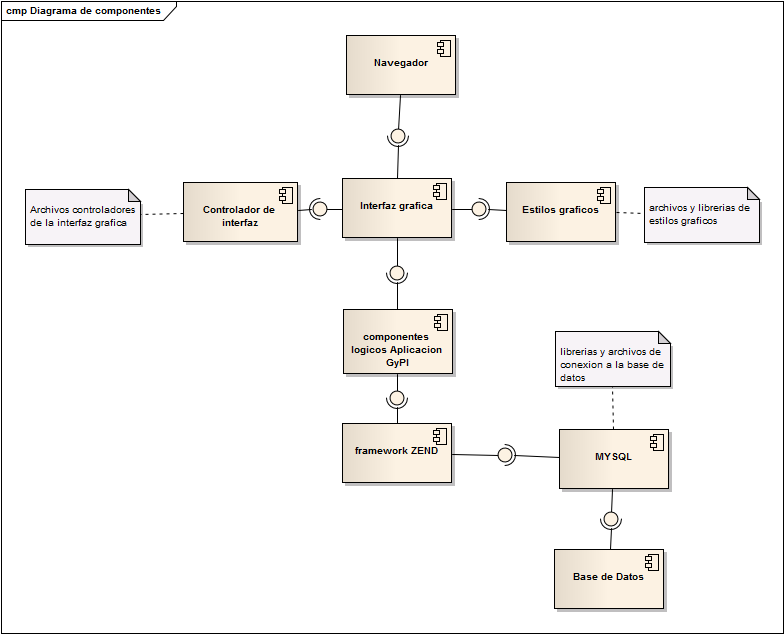
\includegraphics[width=0.75\textwidth]{./img/img9.png}
  \caption{Diagrama de componentes}
\end{figure}


\textbf{Catalogo de elementos}\\


\begin{itemize}
 \item \textbf{Navegador:} Este componente representa el navegador web del cliente para acceder a nuestro sistema. Este componente requiere de ciertos parámetros para su funcionamiento por lo cual se recomienda que se utilicen los navegadores mas comunes como lo son el chrome, firefox ,internet explorer, opera y zafari.
 \item \textbf{Controlador de interfaz:} En el componente controlador de interfaz va a estar el código javascrip que permiten controlar y validar los parámetros ingresados por el usuario a través de la pagina web del sistema logrando así que la información que se envíe al mismo sea una información correcta y procesable.
 \item \textbf{Interfaz gráfica:} En el componente Interfaz gráfica van a estar las pantallas o interfaces que van a interactuar con el usuario. Como va a ser una aplicación web este componente contiene los archivos HTML y PHP encargados de proporcionar las distintas interfaces gráficas.
 \item \textbf{Estilos gráficos:} Este componente contiene los archivos CSS que configuran la apariencia gráfica de las interfaces del sistema.
 \item \textbf{Aplicación GyPI:} Este componente representa el sistema de administración de proyectos de investigación. Es el encargado de gestionar la información de cada uno de los proyectos registrados en el sistema.
 \item \textbf{Framework ZEND:} componente que representa el framework ZEND el cual es un completo entorno de desarrollo integrado para el lenguaje de programación PHP.
 \item \textbf{MySQL:} Este componente se utiliza para realizar la gestión de la base de datos del sistema.
 \item \textbf{Bases de datos:} Este componente representa la base de datos del sistema.
\end{itemize}

\textbf{Variabilidad:}
Los componentes de estilos gráficos pueden ser remplazados por otros componentes que provean una mejor vista estética en caso de ser necesaria.\\
El framework ZEND  puede ser remplazado por otro framework que provea un funcionamiento similar de manera que se pueda configurar correctamente los archivos de conexión a la base de datos y provea la facilidad para organizar correctamente los archivos de configuración y lógica del sistema.\\

\textbf{Razón del diseño:}
Se escogieron componentes de estilos gráficos ya que estos permiten fácilmente aplicar un patrón de diseño a las distintas interfaces que necesite nuestro sistema, brindando una configuración y aplicación de manera fácil, rápida y sencilla.\\
El framewok ZEND fue escogido ya que permite la organización del los archivos del sistema de manera óptima para nuestras necesidades a demás de esto este framework cuenta con una muy buena documentación ya que es ampliamente utilizado por muchos desarrolladores que lo consideran robusto y organizado.\\
\\

\textbf{Vistas relacionadas}
\begin{itemize}
\item Vista de despliegue --- Diagrama de despliegue
\item Vista de diseño --- Diagrama de clases
\end{itemize}

\subsection{Diagrama de paquetes}

% imagen diagrama de paquetes
\begin{figure}[h!]
  \centering
    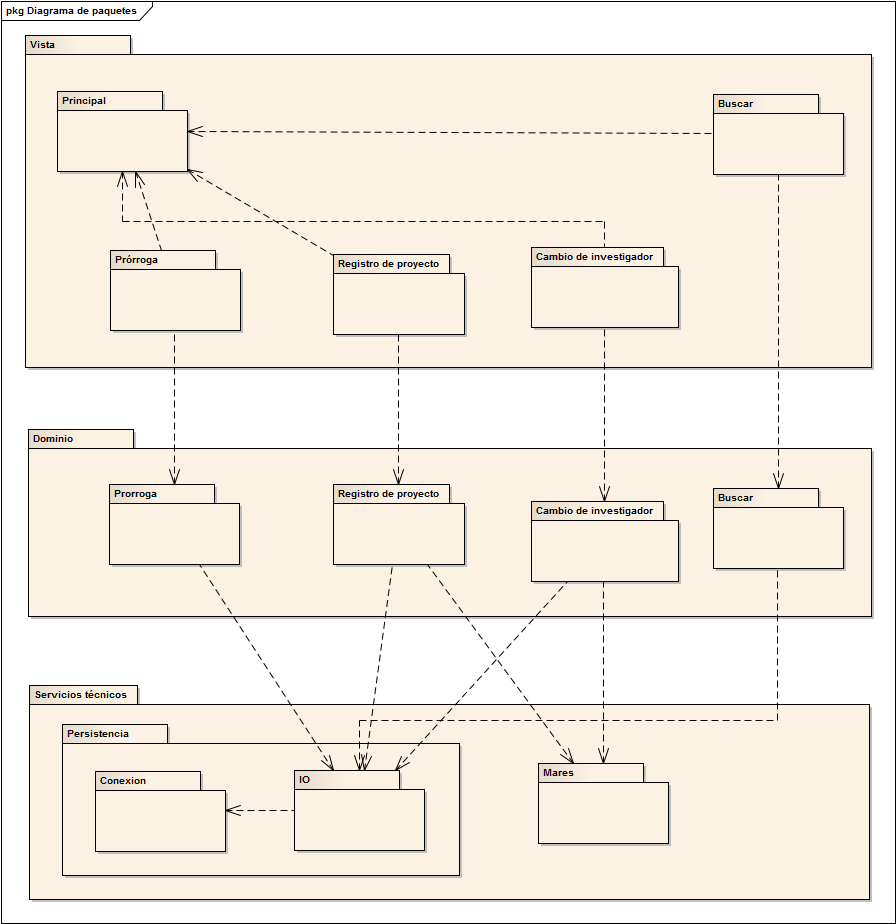
\includegraphics[width=0.75\textwidth]{./img/img10.png}
  \caption{Diagrama de paquetes}
\end{figure}


\textbf{Catalogo de elementos}\\

\begin{itemize}
 \item \textbf{Principal\_vista:} Este modulo representa la interfaz que el sistema proporciona para la comunicación con el usuario. Contiene los archivos HTML,  javascript y CSS con los cuales se desarrolla la interfaz principal del sistema.
 \item \textbf{prórroga\_vista:} En este modulo representa la interfaz gráfica correspondiente a las prórrogas.Contiene los archivos HTML, javascript y CSS con los que se desarrolla la interfaz pertinente a las prórrogas.
 \item \textbf{Registro de Proyecto\_vista:} En este modulo representa la interfaz gráfica para registrar un proyecto de investigación en el sistema. Contiene los archivos HTML, javascript y CSS con los que se desarrolla la interfaz con la que el usuario interactúa con el sistema para el registro de un proyecto de investigación.
 \item \textbf{Cambio de investigador\_vista:} En este modulo representa la interfaz gráfica correspondiente a la solicitud de un cambio de investigador. Contiene los archivos HTML, javascript y CSS con los que se desarrolla la interfaz para solicitar un cambio de investigador y para dar respuesta a las solicitudes pendientes.
 \item \textbf{Consulta\_vista:} Este modulo  representa la interfaz gráfica utilizada para realizar las búsquedas en el sistema.Contiene los archivos HTML, javascript y CSS con los que se desarrolla la interfaz que permite al usuario realizar una búsqueda en el sistema.
 \item \textbf{prórroga\_dominio:} En este modulo se lleva a cabo la lógica del sistema relacionada con las prórrogas. Este modulo contiene las clases PHP que se relacionan con las prórrogas y las clases controladoras del las mismas.
 \item \textbf{Registro de Proyecto\_dominio:} En este modulo se lleva a cabo la lógica del sistema relacionada con el proceso de registro de un proyecto. Este modulo contiene las clases PHP que se relacionan con los proyectos y las clases controladoras del los mismos.
 \item \textbf{Cambio de investigador\_dominio:} En este modulo se lleva a cabo la lógica del sistema relacionada con el proceso de solicitud y respuesta a un cambio de investigador. En este modulo se encuentran las clases PHP relacionadas con un cambio de investigador y su respectivo controlador.
 \item \textbf{Consulta\_dominio:} En este modulo se lleva a cabo la lógica del sistema relacionada con la búsqueda de información en el sistema. Contiene las clases PHP que permiten realizar una búsqueda en el sistema.
 \item \textbf{Conexión:} Este modulo contiene los archivos de conexión a la base de datos del sistema. En este modulo están contenidos los archivos del framework utilizado los cuales nos permiten establecer los parámetros de conexión y configuraron a la base de datos del sistema.
 \item \textbf{IO:} contiene los archivos que utiliza el sistema para el ingreso y consulta los datos en la base de datos.
 \item \textbf{Mares:} Este modulo representa el sistema Mares de la Universidad de Antioquia. Este modulo contiene las clases que permiten la conexión entre el sistema GyPI y Mares necesaria para obtener el vinculo de los integrantes de un proyecto con la Universidad de Antioquia.
\end{itemize}

\textbf{Razón del diseño:}
Utilizamos este diagrama para visualizar de manera clara el patrón de arquitectura de software utilizado, en nuestro caso el Modelo Vista Controlador.\\

\textbf{Vistas relacionadas}
\begin{itemize}
 \item Vista de implementación --- Diagrama de componentes
 \item Vista de diseño --- Diagrama de clases
\end{itemize}


\section{Vista de procesos}

\subsection{Diagrama de actividades}


\subsubsection{Registrar Proyecto}

% Imagen diagrama de actividades
\begin{figure}[h!]
  \centering
    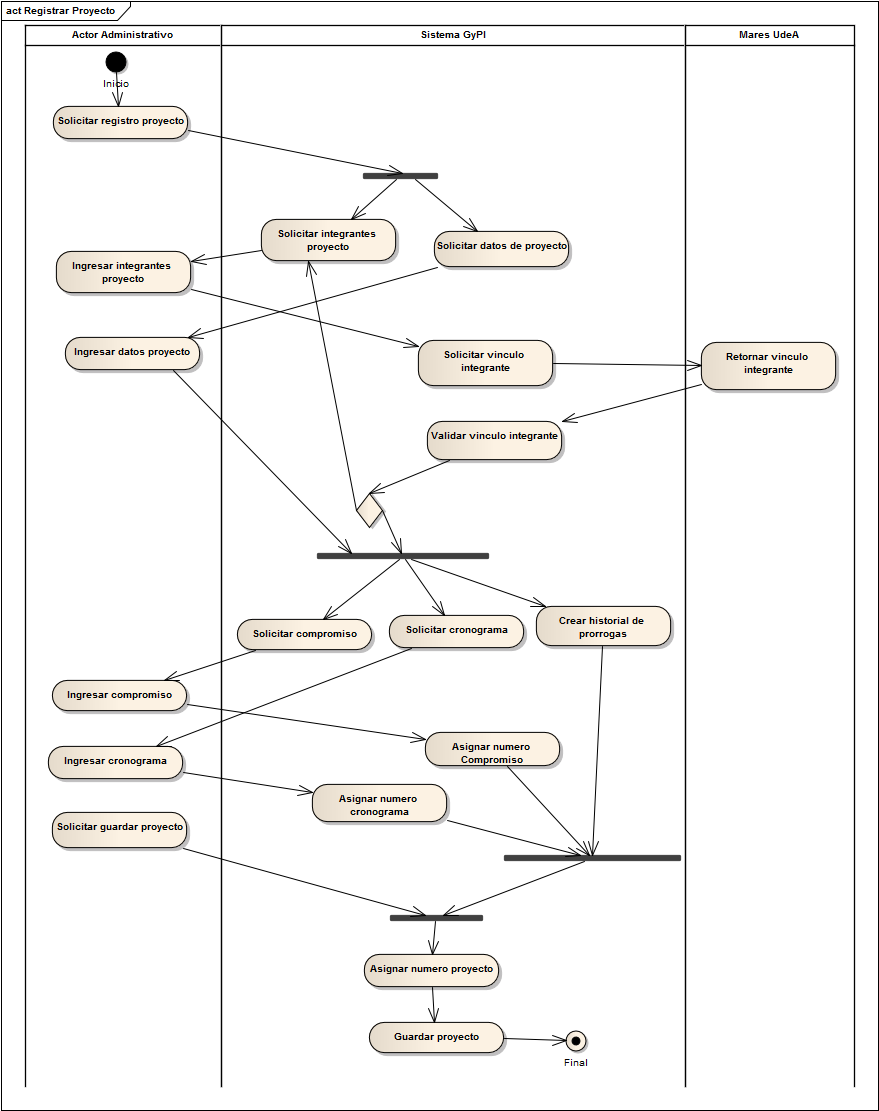
\includegraphics[width=0.75\textwidth]{./img/img11.png}
  \caption{Diagrama de actividades - Registrar proyecto}
\end{figure}


\textbf{Catalogo de elementos}\\

\begin{itemize}
 \item \textbf{solicitar registro proyecto:} El usuario Administrativo solicita registrar un proyecto en el sistema.
 \item \textbf{solicitar integrantes proyecto:} El sistema solicita que se ingresen los integrantes del proyecto.
 \item \textbf{solicitar datos de proyecto:} El sistema solicita que se ingresen los datos del proyecto.
 \item \textbf{ingresar datos de proyecto:} El usuario ingresa los datos del proyecto.
 \item \textbf{ingresar integrantes de proyecto:} El usuario ingresa los integrantes del proyecto.
 \item \textbf{solicitar vinculo integrante:} El sistema solicita el vinculo del integrante a través de la plataforma Mares de la Universidad de Antioquia.
 \item \textbf{retornar vinculo integrante:} El sistema Mares retorna el vinculo del integrante.
 \item \textbf{validar vinculo integrante:} El sistema valida que el integrante tenga algún tipo de vinculo con la universidad.
 \item \textbf{solicitar compromiso:} El sistema solicita los compromisos para el proyecto que esta siendo registrado.
 \item \textbf{solicitar cronograma:} El sistema solicita el cronograma para el proyecto que esta siendo registrado.
 \item \textbf{crear historial de prórrogas:} El sistema crea un nuevo historial de prórrogas vacío para el proyecto que esta siendo registrado.
 \item \textbf{ingresar compromisos:} El usuario ingresa el o los compromisos para este proyecto.
 \item \textbf{ingresar cronograma:} EL usuario ingresa el cronograma para este proyecto.
 \item \textbf{asignar numero compromiso:} El sistema asigna un numero único a cada uno de los compromisos ingresados.
 \item \textbf{asignar numero cronograma:} El sistema asigna un numero único al cronograma registrado.
 \item \textbf{solicitar guardar proyecto:} El usuario solicita guardar el proyecto.
 \item \textbf{asignar numero proyecto:} El sistema asigna un numero único al proyecto.
 \item \textbf{guardar proyecto:} El sistema guarda el proyecto que ha sido registrado.
\end{itemize}

\textbf{Vistas relacionadas}
\begin{itemize}
\item Vista de procesos --- Diagrama de estados
\item Vista de procesos --- Diagrama de secuencias
\end{itemize}

\subsubsection{Responder solicitud de prórroga}

% Imagen diagrama de actividades
\begin{figure}[h!]
  \centering
    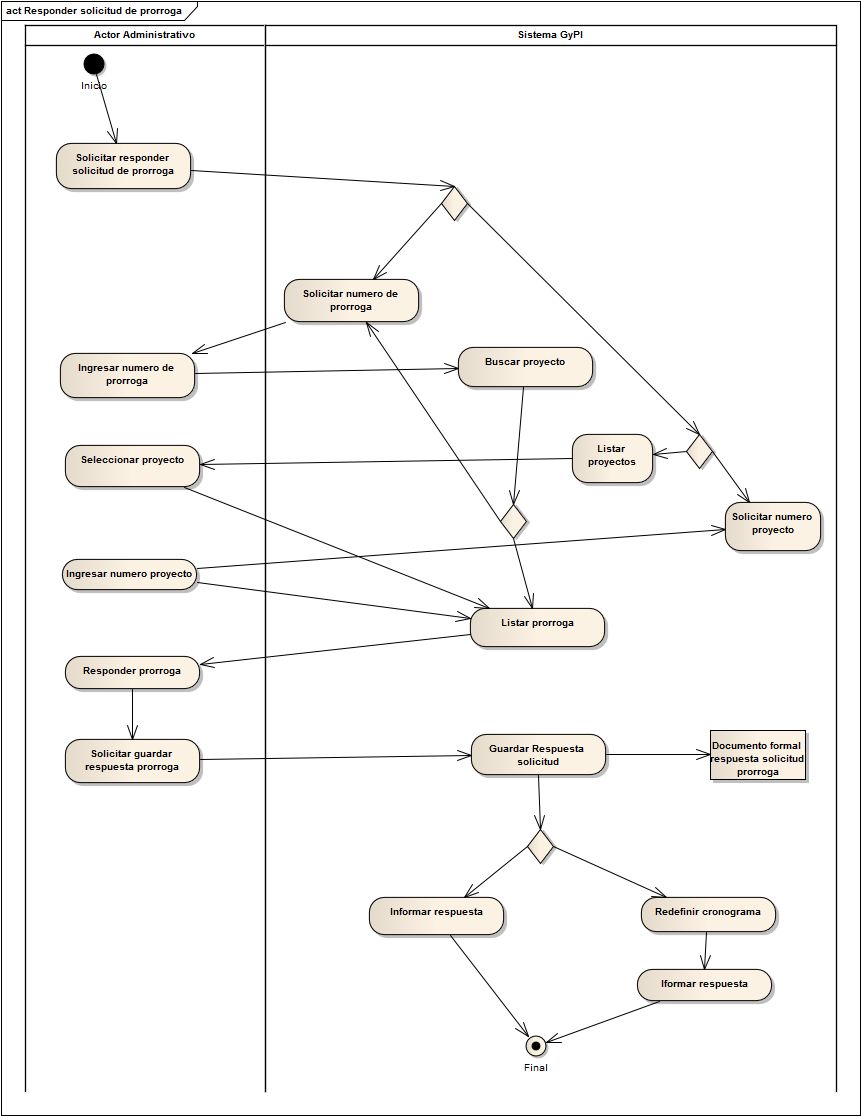
\includegraphics[width=0.75\textwidth]{./img/img12.png}
  \caption{Diagrama de actividades - Responder solicitud de prórroga}
\end{figure}

\textbf{Catalogo de elementos}
\begin{itemize}
  \item \textbf{solicitar responder solicitud de prórroga:} El usuario Administrativo solicita al sistema responder a una solicitud de prórroga.
  \item \textbf{solicitar numero de prórroga:} El sistema brinda la opción de búsqueda a través del numero de la prórroga (opción 1).
  \item \textbf{ingresar numero de prórroga:} El usuario ingresa el numero de la prórroga.
  \item \textbf{buscar proyecto:} El sistema brinda la opción de búsqueda a través de los proyectos (opción 2).
  \item \textbf{listar proyectos:} El sistema lista los proyectos existentes. (opción 2.1).
  \item \textbf{seleccionar proyecto:} El usuario selecciona el proyecto.
  \item \textbf{solicitar numero proyecto:} El sistema solicita el numero de proyecto al cual se le va a responder la solicitud de prórroga (opción 2.2).
  \item \textbf{ingresar numero  proyecto:} El usuario ingresa el numero del proyecto.
  \item \textbf{listar prórroga:} El sistema lista la prórroga que esta pendiente a la respuesta.
  \item \textbf{responder prórroga:} El usuario responde la prórroga.
  \item \textbf{solicitar guardar respuesta prórroga:} El usuario solicita guardar la respuesta de la solicitud de prórroga.
  \item \textbf{guardar respuesta solicitud:} El sistema guarda la respuesta a la solicitud de prórroga.
  \item \textbf{documento formal respuesta solicitud prórroga:} El sistema genera un documento formal con la respuesta y los detalles de la solicitud de prórroga.
  \item \textbf{informar respuesta:} El sistema informa al grupo de investigación sobre la respuesta de la prórroga.
  \item \textbf{redefinir cronograma:} El sistema redefine el cronograma del proyecto si la prórroga es aceptada.
\end{itemize}


\subsubsection{Solicitud de prórroga}

% Imagen diagrama de actividades
\begin{figure}[h!]
  \centering
    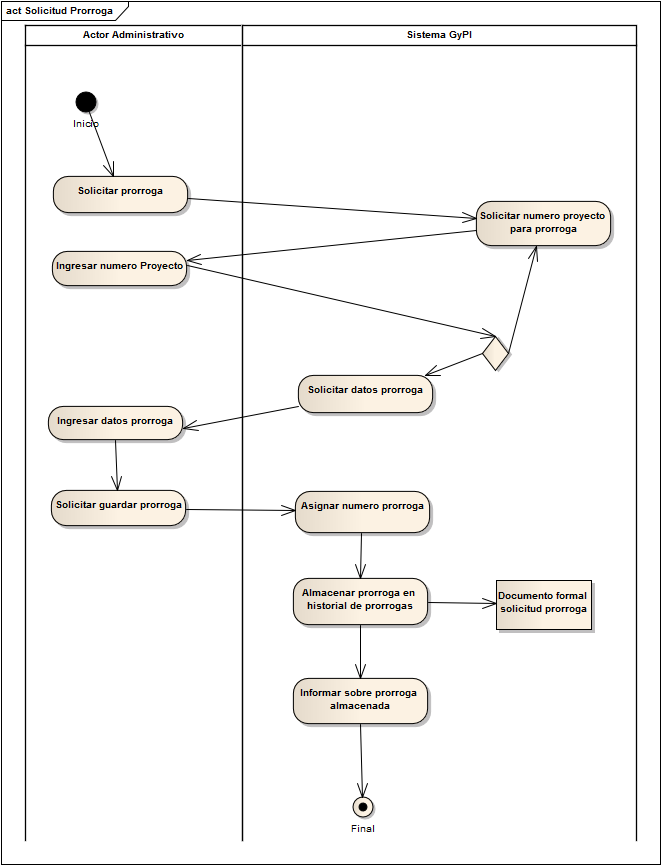
\includegraphics[width=0.75\textwidth]{./img/img13.png}
  \caption{Diagrama de actividades - solicitud de prórroga}
\end{figure}

\textbf{Catalogo de elementos}

\begin{itemize}
\item \textbf{solicitud prórroga:} El usuario Administrativo solicita ingresar una solicitud de prórroga.
\item \textbf{solicitar numero de proyecto para prórroga:} El sistema solicita el numero de proyecto al cual se le va a solicitar una prórroga.
\item \textbf{ingresar numero de proyecto:} El usuario ingresa el numero del proyecto.
\item \textbf{solicitar datos prórroga:} El sistema solicita los datos necesarios para la solicitud de la prórroga
\item \textbf{ingresar datos prórroga:} El usuario ingresa los datos pedidos sobre la solicitud de prórroga.
\item \textbf{solicitar guardar prórroga:} El usuario solicita guardar la solicitud de prórroga.
\item \textbf{asignar numero de prórroga:} El sistema asigna un numero único a la solicitud de prórroga.
\item \textbf{almacenar prórroga en historial de prórrogas:} El sistema almacena la solicitud de prórroga en el historial de prórrogas.
\item \textbf{documento formal solicitud de prórroga:} El sistema genera un documento formal sobre la solicitud de la prórroga.
\item \textbf{informar sobre prórroga almacenada:} El sistema informa que la prórroga ha sido almacenada.
\end{itemize}


\textbf{Vistas relacionadas}
\begin{itemize}
\item Vista de procesos --- Diagrama de estados
\item Vista de procesos --- Diagrama de secuencias
\end{itemize}


\subsubsection{Tramitar compromiso}

% Imagen diagrama de actividades
\begin{figure}[h!]
  \centering
    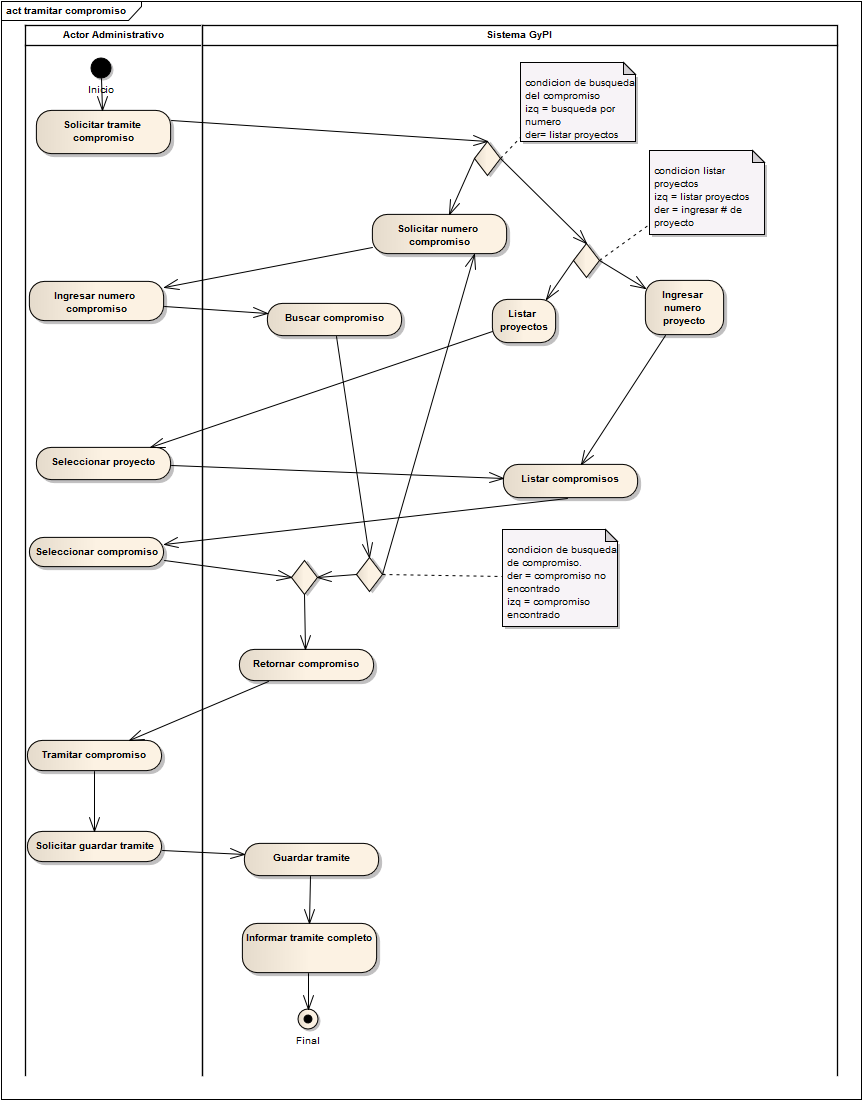
\includegraphics[width=0.75\textwidth]{./img/img14.png}
  \caption{Diagrama de actividades - Tramitar compromiso}
\end{figure}

\textbf{Catalogo de elementos}

\begin{itemize}
 \item \textbf{solicitar tramite compromiso:} El usuario administrativo solicita tramitar un compromiso
 \item \textbf{solicitar numero compromiso:} El sistema solicita en numero de compromiso a tramitar (opción 1)
 \item \textbf{ingresar numero compromiso:} El usuario ingresa el numero de compromiso a tramitar.
 \item \textbf{buscar compromiso:} El sistema busca el compromiso según el numero ingresado
 \item \textbf{listar proyectos:} El sistema lista los proyectos registrados (opción 2.1)
 \item \textbf{seleccionar proyecto:} El usuario selecciona el proyecto al cual desea tramitarle el compromiso
 \item \textbf{ingresar numero de proyecto:} El sistema solicita el numero del proyecto al cual se le desea tramitar el compromiso (opción 2.2)
 \item \textbf{listar compromisos:} El sistema lista los compromisos del proyecto
 \item \textbf{seleccionar compromiso :} El usuario selecciona el compromiso que desea tramitar.
 \item \textbf{retornar compromiso:} El sistema retorna el compromiso  ser tramitado.
 \item \textbf{tramitar compromiso:} El usuario tramita el compromiso.
 \item \textbf{solicitar guardar tramite :} El usuario solicita guardar el tramite del compromiso.
 \item \textbf{guardar tramite:} El sistema guarda el tramite del compromiso.
 \item \textbf{informar tramite completo:} El sistema informa que el tramite ha sido completado.
\end{itemize}


\textbf{Vistas relacionadas}
\begin{itemize}
 \item Vista de procesos --- Diagrama de estados
 \item Vista de procesos --- Diagrama de secuencias
\end{itemize}


\subsection{Diagrama de secuencias}

\subsubsection{Registrar solicitud de prórroga}

% imagen diagrama de secuencias
\begin{figure}[h!]
  \centering
    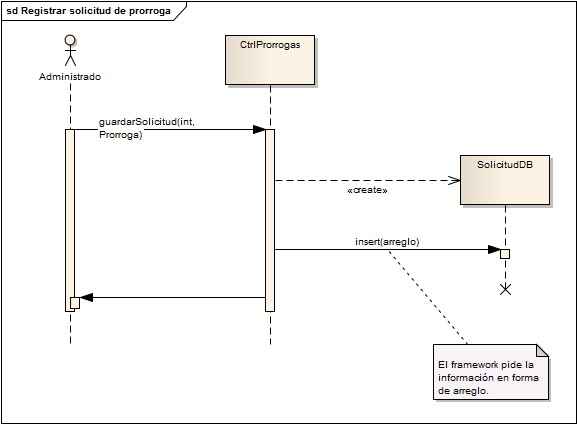
\includegraphics[width=0.75\textwidth]{./img/img15.png}
  \caption{Diagrama de secuencias - Registrar solicitud de prórroga}
\end{figure}

\textbf{Catalogo de elementos}

\begin{itemize}
 \item \textbf{CtrlProrrogas:} Controlador encargado de recibir peticiones de la interfaz gráfica relacionadas con las prorrogas.
 \item \textbf{SolicitudDB:} Clase encargada de cominicarse con la base de datos, mas específicamente con la tabla \textit{tb\_solicitud}, para guardar, actualizar y seleccionar.
\end{itemize}


\textbf{Vistas relacionadas}
\begin{itemize}
 \item Vista de procesos --- Diagrama de estados
 \item Vista de procesos --- Diagrama de actividades
\end{itemize}

\subsubsection{Registro de proyecto}

% imagen diagrama de secuencias
\begin{figure}[h!]
  \centering
    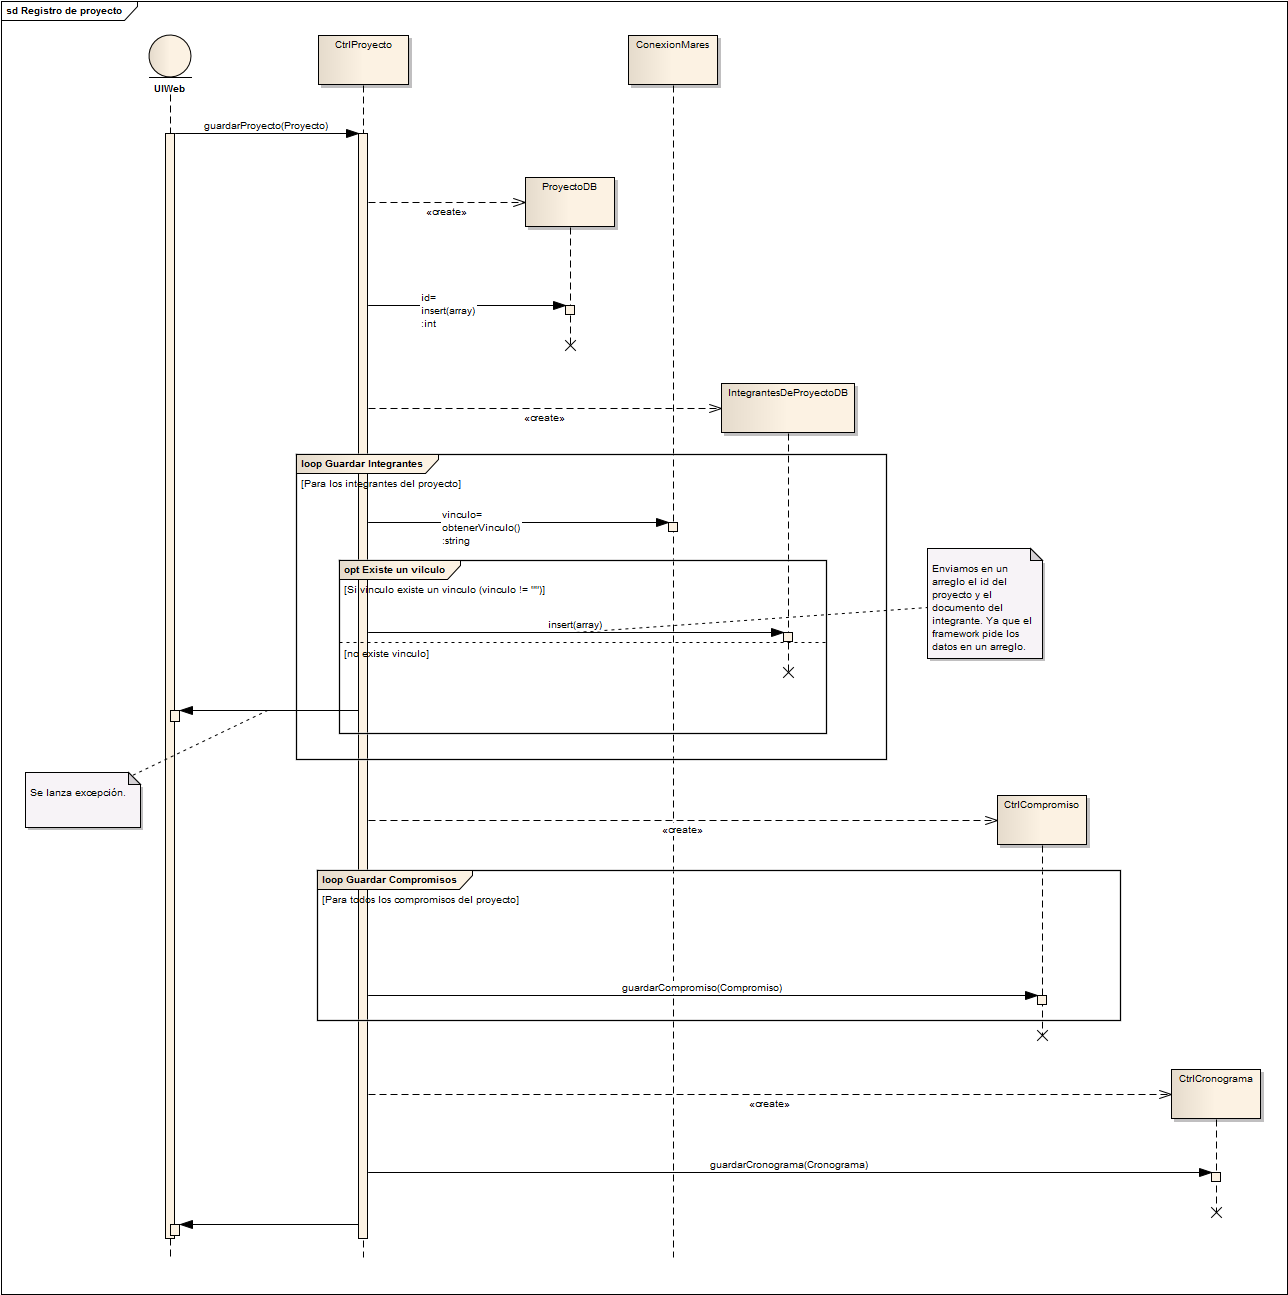
\includegraphics[width=0.75\textwidth]{./img/img16.png}
  \caption{Diagrama de secuencias - Registro de proyecto}
\end{figure}

\textbf{Catalogo de elementos}

\begin{itemize}
 \item \textbf{CtrlProyecto:} Controlador encargado de recibir peticiones de la interfaz gráfica relacionadas con los proyectos.
 \item \textbf{ProyectoDB:} Clase encargada de cominicarse con la base de datos, mas especificamente con la tabla \textit{tb\_proyecto}, para guardar, actualizar y seleccionar.
 \item \textbf{ConexionMares:} Clase que implementa el patrón \textit{facade}, y se encarga de conectarse con el sistema externo Mares para averiguar el vinculo de una persona con la universidad.
 \item \textbf{IntegrantesDeProyectoDB:} Clase encargada de cominicarse con la base de datos, mas especificamente con la tabla \textit{tb\_integrante\_proyecto}, para guardar, actualizar y seleccionar.
 \item \textbf{CtrlCompromiso:} Controlador encargado de ejecutar acciones sobre los compromisos de un proyecto.
 \item \textbf{CtrlCronograma:} Controlador encargado de ejecutar acciones sobre el cronograma de un proyecto.
\end{itemize}

\textbf{Vistas relacionadas}
\begin{itemize}
 \item Vista de procesos --- Diagrama de estados
 \item Vista de procesos --- Diagrama de actividades
\end{itemize}

\subsubsection{Solicitar cambio de investigador}

% imagen diagrama de secuencias
\begin{figure}[h!]
  \centering
    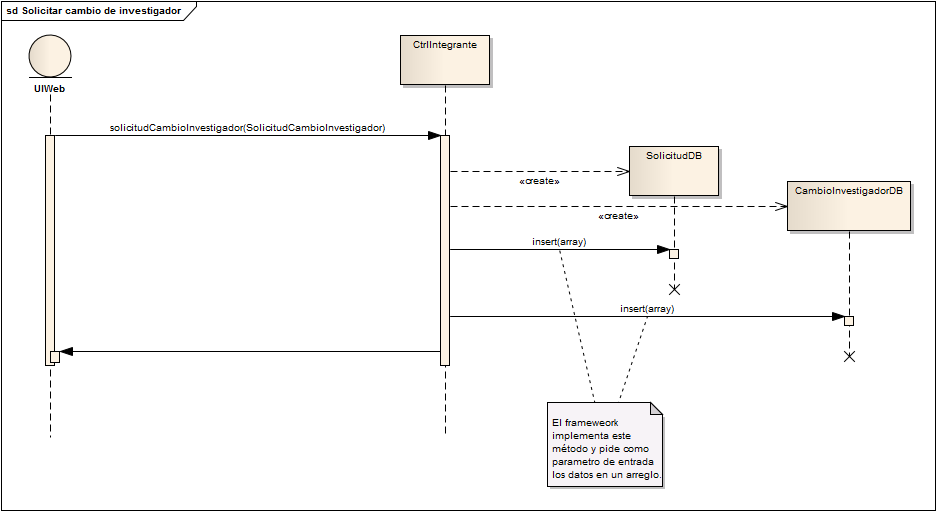
\includegraphics[width=0.75\textwidth]{./img/img17.png}
  \caption{Diagrama de secuencias - Solicitar cambio de investigador}
\end{figure}

\textbf{Catalogo de elementos}

\begin{itemize}
 \item \textbf{CtrlIntegrante:} Controlador encargado de recibir peticiones de la interfaz gráfica relacionadas con los integrantes.
 \item \textbf{SolicitudDB:} Clase encargada de cominicarse con la base de datos, mas especificamente con la tabla \textit{tb\_solicitud}, para guardar, actualizar y seleccionar.
 \item \textbf{CambioInvestigadorDB:} Clase encargada de cominicarse con la base de datos, mas especificamente con la tabla \textit{tb\_cambio\_investigador}, para guardar, actualizar y seleccionar.
\end{itemize}

\textbf{Vistas relacionadas}
\begin{itemize}
 \item Vista de procesos --- Diagrama de estados
 \item Vista de procesos --- Diagrama de actividades
\end{itemize}


\subsubsection{Validar compromiso}

% imagen diagrama de secuencias
\begin{figure}[h!]
  \centering
    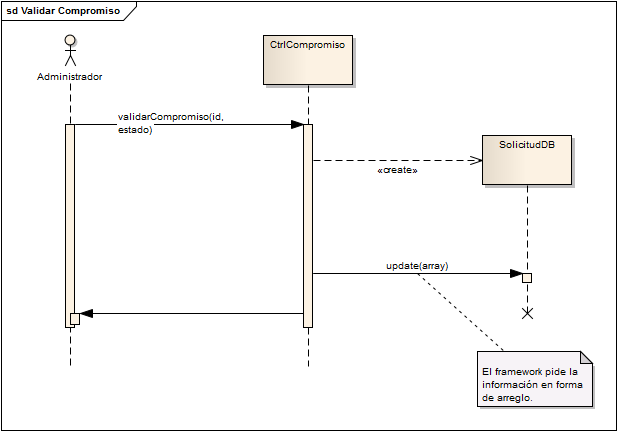
\includegraphics[width=0.75\textwidth]{./img/img18.png}
  \caption{Diagrama de secuencias - Validar compromiso}
\end{figure}

\textbf{Catalogo de elementos}
\begin{itemize}
 \item \textbf{CtrlCompromiso:} Controlador encargado de recibir peticiones de la interfaz gráfica relacionadas con los integrantes.
 \item \textbf{SolicitudDB:} Clase encargada de cominicarse con la base de datos, mas especificamente con la tabla \textit{tb\_solicitud}, para guardar, actualizar y seleccionar.
\end{itemize}

\textbf{Vistas relacionadas}
\begin{itemize}
 \item Vista de procesos --- Diagrama de estados
 \item Vista de procesos --- Diagrama de actividades
\end{itemize}


\subsection{Diagrama de estados}


\subsubsection{Cambio de investigador}

% imagen diagrama de estados
\begin{figure}[h!]
  \centering
    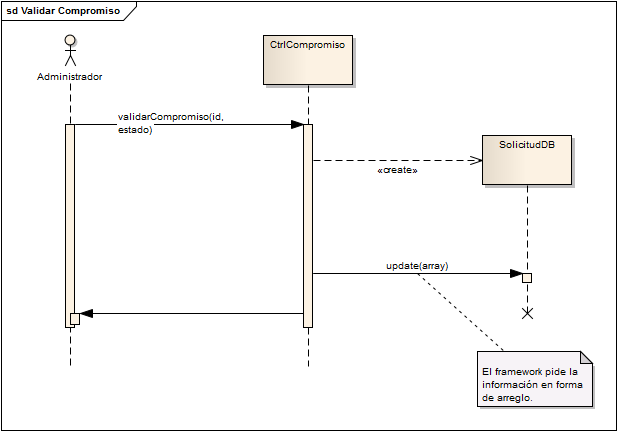
\includegraphics[width=0.75\textwidth]{./img/img19.png}
  \caption{Diagrama de estados - Cambio de investigador}
\end{figure}

\textbf{Catalogo de elementos}

\begin{itemize}
 \item \textbf{solicitado:} Este es el estado inicial de un cambio de investigador el cual fue solicitado en el sistema mediante la solicitud de un cambio de investigador.
 \item \textbf{Evaluado:} Este estado evalúa el perfil del investigador candidato para el cambio. En este estado se evalúa que el candidato cumpla con los requisitos mínimos para sustituir el instigador que actualmente esta en el proyecto al cual se le requiere hacer el cambio de investigador.
 \item \textbf{Aceptado:} Este estado indica que el investigador candidato cumple con los requisitos mínimos para ser investigador y por ende se procede a realizar el remplazo
 \item \textbf{rechazado:} Este estado indica que el candidato a investigador no cumple con los requisitos mínimos para ser investigador y por ende se rechaza. En este estado se da la posibilidad de redefinir el perfil del candidato o sustituir el mismo para realizar una nueva solicitud.
 \item \textbf{Redefinido:} En este estado se redefine el perfil del candidato a ser investigador para nuevamente solicitar en cambio.
\end{itemize}



\textbf{Vistas relacionadas}
\begin{itemize}
 \item Vista de procesos --- Diagrama de actividades
\end{itemize}



\subsubsection{Solicitud prórroga}

% imagen diagrama de estados
\begin{figure}[h!]
  \centering
    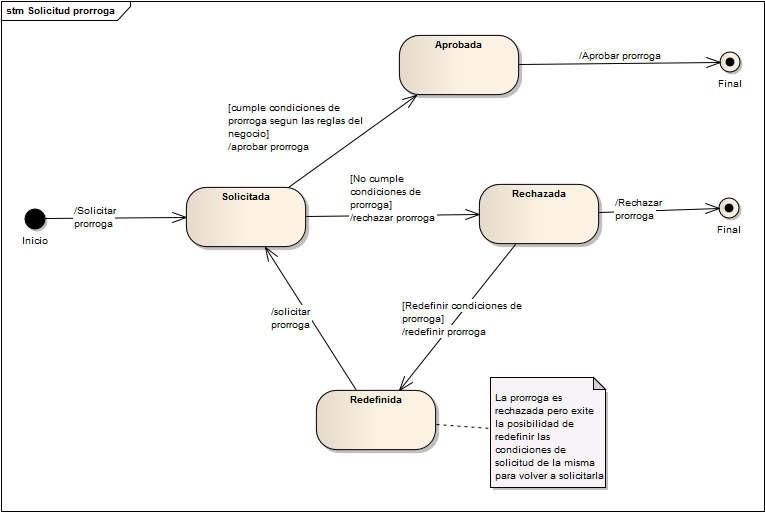
\includegraphics[width=0.75\textwidth]{./img/img20.png}
  \caption{Diagrama de estados - Solicitud prórroga}
\end{figure}

\textbf{Catalogo de elementos}

\begin{itemize}
 \item \textbf{solicitada:} Este es el estado inicial de una solicitud de prórroga la cual fue realizada mediante el sistema.
 \item \textbf{aprobada:} Este estado indica que la prórroga ha sido aprobada ya que cumple con los requisitos mínimos para que sea aprobada y con las reglas del negocio RN-006 prórrogas, RN-007 Solicitud  prórroga
 \item \textbf{rechazada:} Este estado indica que la solicitud de prórroga no cumple con los requisitos mínimos para que sea aprobada o no cumple con la regla de negocio RN-006 prórrogas. En este estado se la la posibilidad de que los términos en la solicitud de una prórroga sea cambiado para realizar una nueva solicitud.
 \item \textbf{redefinida:} En este estado se redefinen los términos de una solicitud de prórroga rechazada para realizar una nueva solicitud.
\end{itemize}


\textbf{Vistas relacionadas}
\begin{itemize}
 \item Vista de procesos --- Diagrama de actividades
\end{itemize}


\subsubsection{Compromiso}

% imagen diagrama de estados
\begin{figure}[h!]
  \centering
    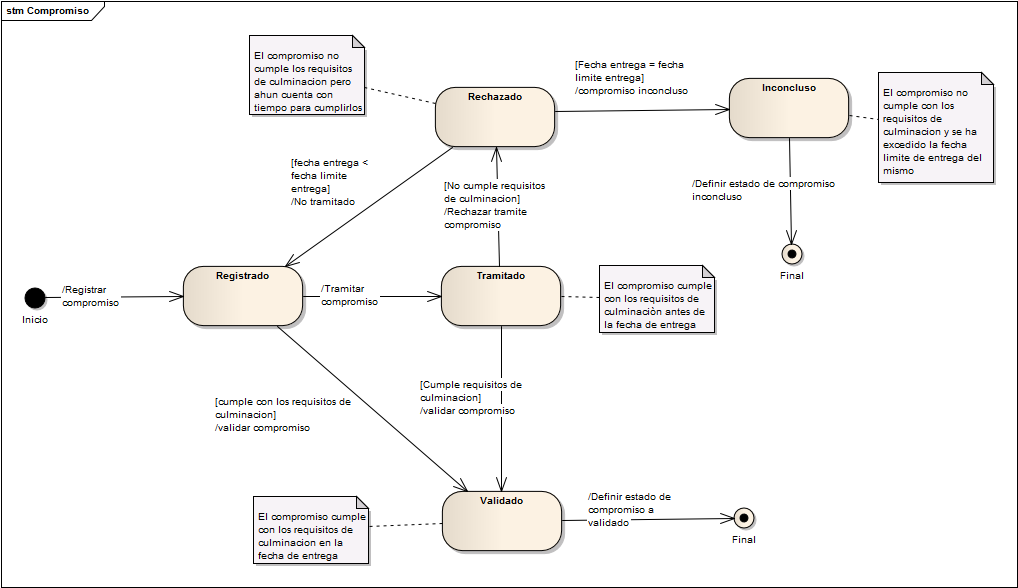
\includegraphics[width=0.75\textwidth]{./img/img21.png}
  \caption{Diagrama de estados - Compromiso}
\end{figure}

\textbf{Catalogo de elementos}
\begin{itemize}
 \item \textbf{registrado:} Este es el estado inicial de un compromiso  el cual ha sido registrado al registrar un proyecto.
 \item \textbf{Tramitado:} Este estado indica que el compromiso ha sido terminado antes del plazo estipulado para la culminación del proyecto al cual esta asociado.
 \item \textbf{Validado:} Este estado indica que el compromiso ha sido terminado en la fecha planteada para la culminación del proyecto de investigación al cual esta asociado
 \item \textbf{rechazado:} Este estado indica que el compromiso no cumple con los requisitos mínimos para ser validado o tramitado. En el caso en que la fecha de entrega del proyecto aun no haya sido sobrepasada el requisito pasará a estar registrado.
 \item \textbf{Inconcluso:} Este estado indica que el compromiso no cumplió con los requisitos mínimos para ser validado y sobrepaso la fecha limite de culminación del proyecto por ende se define inconcluso.
\end{itemize}





\textbf{Vistas relacionadas}
\begin{itemize}
 \item Vista de procesos --- Diagrama de actividades
\end{itemize}


\subsection{Vista de despliegue}

\subsubsection{Diagrama de despliegue}

% imagen diagrama de despliegue
\begin{figure}[h!]
  \centering
    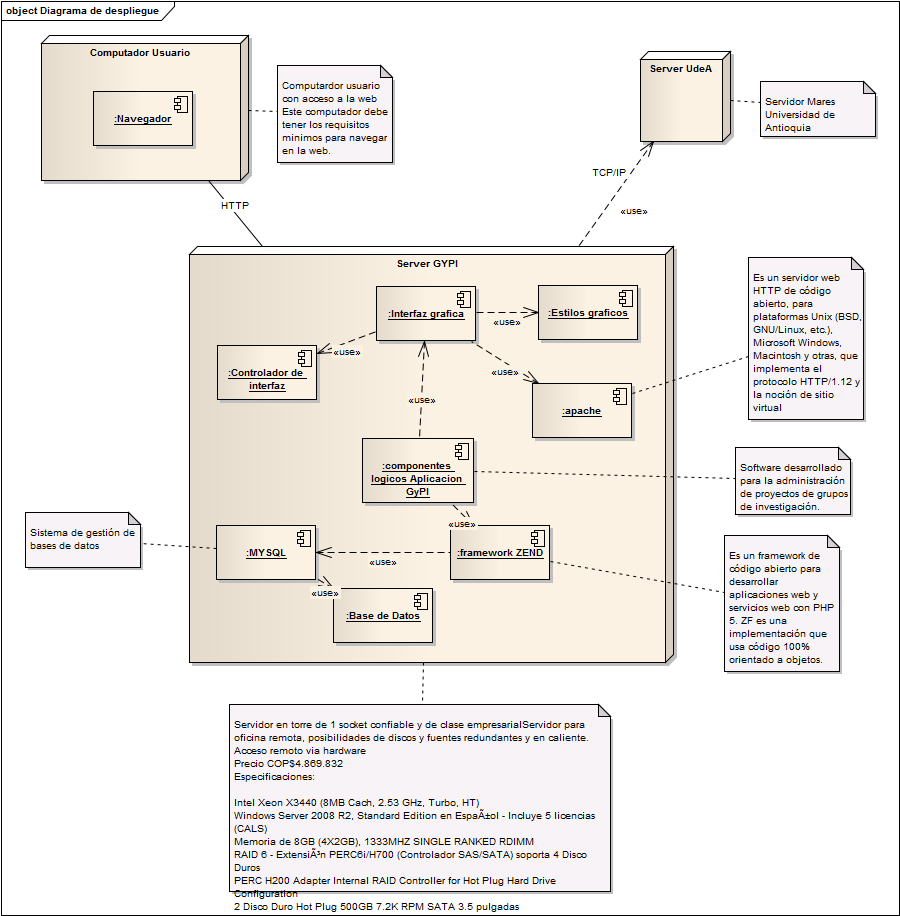
\includegraphics[width=0.75\textwidth]{./img/img22.png}
  \caption{Vista de despliegue}
\end{figure}

\textbf{Catalogo de elementos}

\begin{itemize}
 \item \textbf{Computador usuario:} Representa los equipos de los usuarios del sistema. Estos equipos deben cumplir con los requisitos mínimos para acceder a una pagina web y contar con la capacidad de instalar los diversos plugins para la correcta visualización de la misma. El equipo del usuario se conecta con el servidor a través de el protocolo HTTP.
 \item \textbf{Server UdeA:} Representa el sistema Mares de la universidad de Antioquia al cual el sitema GyPI realiza las peticiones para obtener los vincuos de los usuarios que van a ser registrados en un grupo de investigación. Esta conexión se realiza mediante el protocolo TCP/IP el cual tiene un alto grado de fiabilidad y es muy eficiente en redes con volumen de trafico grande.
 \item \textbf{Server GyPI:} Representa el servidor del sistema GyPI, es un servidor Intel Xeon X3440 (8MB de cache, 2,5GHz) implementa un sistema operativo Windows server 2008, contiene 8 GB de memoria ram, soporta 4 discos duros y contiene un adaptador Gigabit Ethernet integrado de doble puerto. En este servidor estaran almacenados los componentes de la parte gráfica y lógica del sistema a demás de la base de datos del mismo. La comunicación con la base de datos se realiza  a través del framework de ZEND y este mediante sus archivo de configuración application.ini nos permite determinar los parámetros para la conexión.
\end{itemize}


\textbf{Razón del diseño:}
El sistema GyPI debe contar con un servidor de muy buen desempeño y de respuesta óptima. La capacidad de almacenamiento de los datos y la fiabilidad de la persistencia de los mismos debe ser fundamental puesto que se trata de un proceso sumamente importante para la Universidad es por eso que el servidor elegido brinda una amplia capacidad de almacenamiento y seguridad en los datos alojados en este.

\textbf{Vistas relacionadas}
\begin{itemize}
 \item Vista de implementación --- diagrama de componentes
\end{itemize}



\subsection{Vista de sistemas}

\subsubsection{Diagrama de secuencia sistema GyPI – Mares}

% imagen diagrama de secuencia 
\begin{figure}[h!]
  \centering
    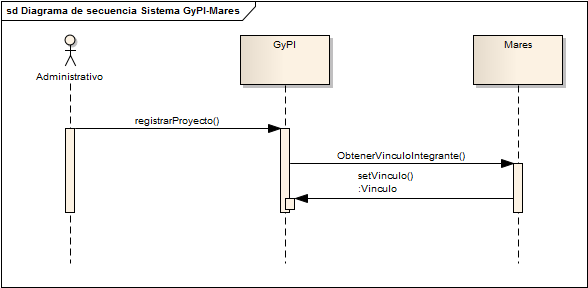
\includegraphics[width=0.75\textwidth]{./img/img23.png}
  \caption{Diagrama de secuencia sistema GyPI – Mares}
\end{figure}

La interacción entre el sistema GyPI y Mares de la Universidad de Antioquia se da para obtener el vinculo que un posible integrante de un proyecto de investigación tiene con la Universidad.

\textbf{Catalogo de elementos}

\begin{itemize}
 \item \textbf{Administativo:} Usuario encargado de registrar un proyecto de investigación.
 \item \textbf{GyPI:} Sistema para la gestión de proyectos de investigación. Este sistema solicita a el sistema Mares de la Universidad de Antioquia el vinculo que un integrante posee con esta para poder registrar a este en un determinado proyecto de investigación.
 \item \textbf{Mares:} Sistema de la Universidad de Antioquia en el cual se encuentra la información acerca de las personas que tienen algún tipo de vinculo con la misma.
\end{itemize}

\textbf{Vistas relacionadas}
\begin{itemize}
 \item Vista de despliegue --- Diagrama de despliegue
 \item Vista de procesos --- Diagrama de secuencias.
\end{itemize}


\chapter{Gestión y soporte}
\section{Gestión}
\subsection{Lecciones aprendidas del diseño}

\begin{itemize}
 \item El modelo de diseño nos ayudó de manera precisa a preconcebir el funcionamiento del sistema y determinar de manera acertada la mejor forma para desarrollar el mismo. Este modelo nos permitió mostrar al cliente la manera como el sistema se va a comportar frente a diversas situaciones logrando así que el cliente visualice el funcionamiento del sistema de manera previa y aclare los conceptos que quizás no hayan sido bien concebidos en la especificación de los requisitos o en el modelo del negocio. 
 \item El modelo de diseño nos brinda una etapa previa a la codificación de la aplicación, etapa que en muchos casos los desarrolladores de software solemos omitir ya que creemos tener certeza sobre lo que se nos ha pedido desarrollar e iniciamos a codificar la aplicación cuando en realidad quizás ni sabemos hacia donde pretendemos llegar con la misma. El modelado de diseño nos ayuda a concebir los componentes necesarios para el desarrollo del sistema y la forma en como cada uno de ellos interactúa, esto es muy importante ya que nos reduce en gran medida los componentes innecesarios o redundantes.
 \item Realizar un buen modelo de diseño nos permite identificar el patrones de diseño que mejor se adaptan al sistema. Identificar un buen patrón  nos permite reducir el acoplamiento que se puede llegar a dar en el sistema, ayuda a que a la hora de implementar un cambio en el sistema no implique rediseñar el mismo sino que por el contrario se haga el cambio de manera fácil y efectiva. Un buen patrón de diseño aumenta la mantenibilidad del sistema y lo hace mucho mas flexible permitiendo que este pueda adaptarse a los cambios que pueda llegar a tener.
 \item El modelo de diseño se fundamenta en gran parte en el modelo de negocios y el modelo de requisitos, el tener errores en alguno de estos diseños acarrea errores en el modelo del diseño de manera que quizás sea necesario regresar a redefinir los requisitos o la concepción del sistema, lo cual incurriría en gastos de tiempo y monetarios para los desarrolladores. Diseñar de manera adecuada y consistente los modelos previos al modelo de diseño nos ayuda tener un sistema mas solido y adecuado para nuestro cliente puesto que muchos de los errores que se presentan en el desarrollo de aplicaciones se dan el la concepción de los requisitos o en el diseño del sistema.
 \item El modelo de diseño nos describe la estructura de un sistema de forma detallada permitiendo que el desarrollador aborde el desarrollo del sistema de manera óptima puesto que al conocer la estructura del sistema mediante los distintos diagramas que nos brinda el modelo de diseño se conoce de manera clara el comportamiento de cada uno de los componentes del sistema frente a las interacciones que un usuario pueda tener con el mismo, logrando una respuesta óptima y eficiente del sistema a las necesidades que el mismo pretende suplir.
 \item Realizar una correcta documentación sobre los procesos desarrollados en cada una de las etapas del modelado del sistema facilitan la comprensión y manejo de la aplicación a personas que ajenas al desarrollo de la misma. Documentar el desarrollo de la aplicación y cada uno de los procesos llevados a cabo en la misma facilita el mantenimiento de esta reduciendo de manera notable el tiempo necesario para la comprensión de la misma al igual que se ayuda a que no se realicen procesos que quizás ya estén implementados en la aplicación y que por el desconocimiento del proceso de desarrollo e la misma se haga necesarios realizar.
\end{itemize}

\subsection{Indicadores de gestión}
\subsubsection{Desviación de lo planeado vs lo ejecutado}

\begin{figure}[h!]
  \centering
    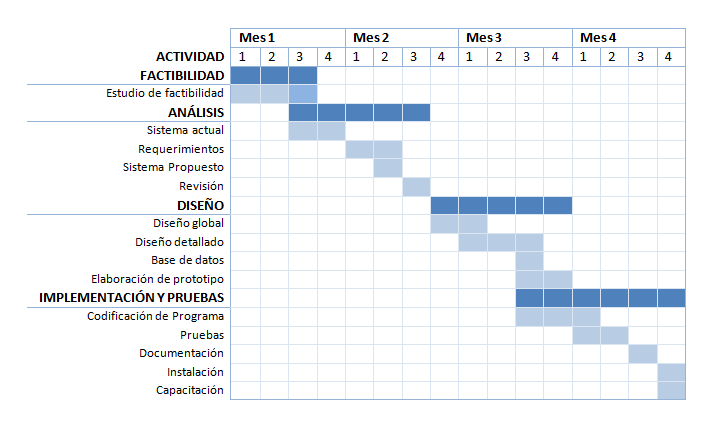
\includegraphics[width=0.75\textwidth]{./img/cal1.png}
  \caption{Plan de trabajo propuesto}
\end{figure}
 
\begin{figure}[h!]
  \centering
      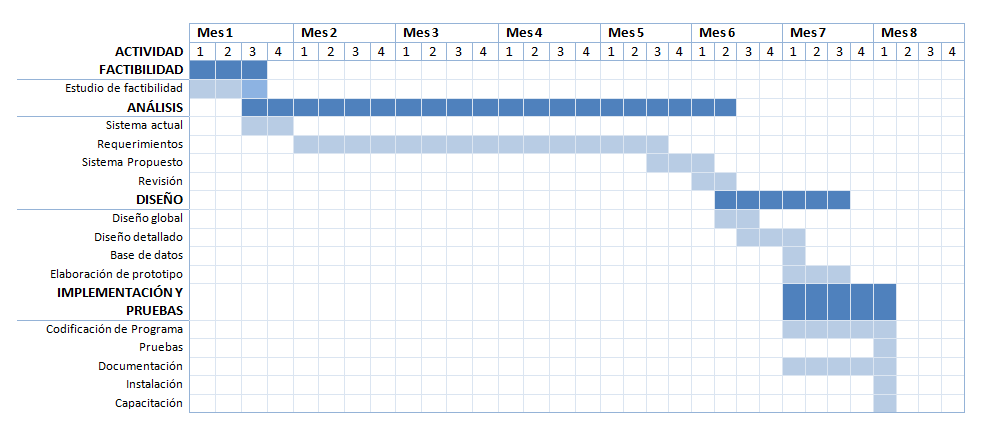
\includegraphics[width=0.75\textwidth]{./img/cal2.png}
  \caption{Plan de trabajo ejecutado}
\end{figure}

\maketitle En las figuras 3.1 y 3.2 podemos observar el plan propuesto al inicio del proyecto con el ejecutado. El desvío se devió a la situación que en ese momento ocurrida en la Universdad de Antioquia. Por esta razón el cliente pidió parar el desarrollo normal del proyecto hasta que se normalizara la situación y los estudiantes, profesores y grupos de investigación regresaran a su normal funcionamiento.

\subsubsection{Gráfica de valor ganado de proyecto}

Acontinuacion realizamos una tabla que nos permite visualizar la realcion del presupuesto planteada en
el modelo del nogocio a traves del tiempo estimado de desarrollo de la aplicacion.

\begin{figure}[h!]
  \centering
      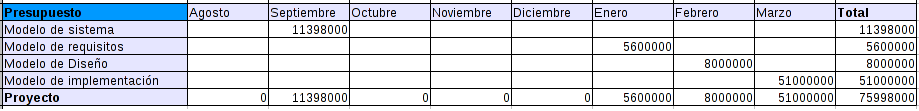
\includegraphics[width=0.75\textwidth]{./img/imagen1.png}
  \caption{Presupuesto}
\end{figure}

La siguiente tabla muestra el porcentaje de avance del proyecto a lo largo del tiempo establecido para el desarrollo del mismo.

\begin{figure}[h!]
  \centering
      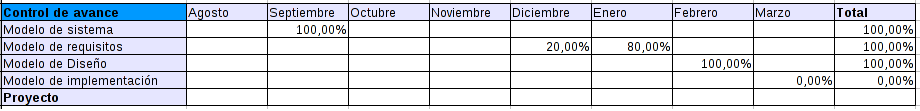
\includegraphics[width=0.75\textwidth]{./img/imagen2.png}
  \caption{Control de avance}
\end{figure}

Se obtiene mediante el calculo del producto entre el porcentaje de avance y el costo presupuestado

\begin{figure}[h!]
  \centering
      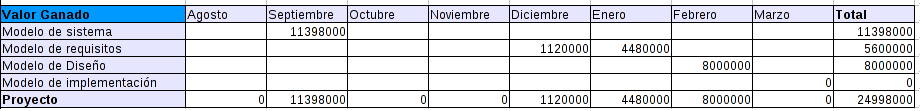
\includegraphics[width=0.75\textwidth]{./img/imagen3.png}
  \caption{Valor ganado}
\end{figure}

La siguiente tabla muestra el costo real de la aplicacion dado que la Universidad de Antioquia estubo cerrada por al rededor de 2 meses lo cual incurre en sobrecostos para el desarrollo del proyecto.

\begin{figure}[h!]
  \centering
      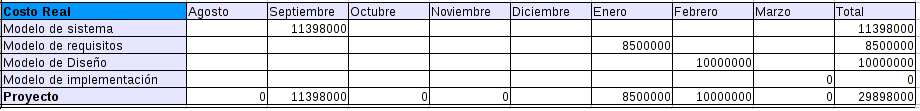
\includegraphics[width=0.75\textwidth]{./img/imagen4.png}
  \caption{Costo real}
\end{figure}

\begin{figure}[h!]
  \centering
      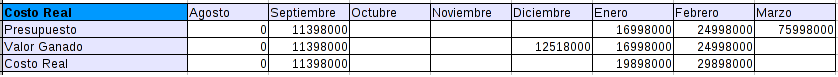
\includegraphics[width=0.75\textwidth]{./img/imagen5.png}
  \caption{Tabla de presupuesto}
\end{figure}

La siguiente grafica muestra el presupuesto pactado en el modelo del negocio contra el costo real para el desarrollo de la aplicacion

\begin{figure}[h!]
  \centering
      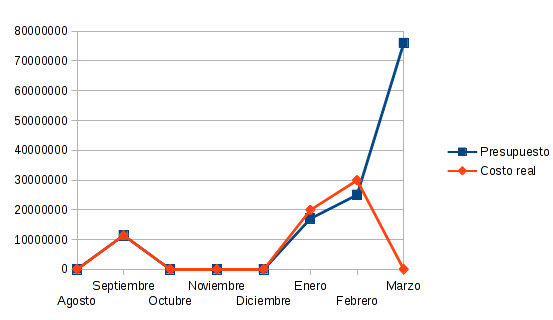
\includegraphics[width=0.75\textwidth]{./img/imagen6.png}
  \caption{Gráfica de valor ganado}
\end{figure}


\section{Soporte}

\subsection{Número de defectos de diseño hallados en verificación y validación}

\begin{figure}[h!]
  \centering
    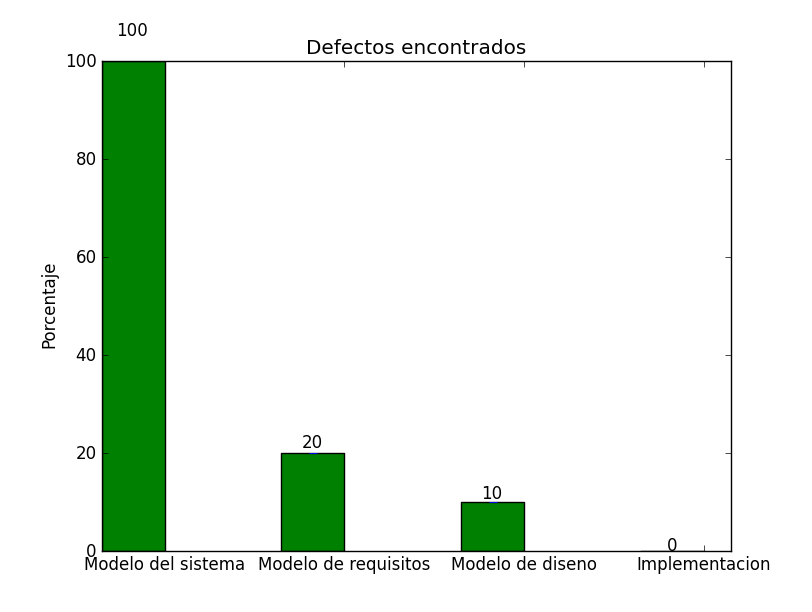
\includegraphics[width=0.75\textwidth]{./img/barras/barras.png}
  \caption{Defectos encontrados}
\end{figure}

\maketitle Como podemos ver en a figura 3.9, los errores encontrados en el modelo del sistema fueron de un 100\%, ya que luego de esta entrega, el sistema fue dividido en dos por su complegidad. El primer módulo se orientó en la parte administrativa, la cual es la que trabajamos en este documento, y el segundo módulo, se orientó a la parte presupiestal. En el modelo de requisitos y de diseño encontramos un 20\% y 10\% respectivamente, devido a problemas de comunicación con el cliente y el equipo de desarrollo. La implementación cuenta con 0\% de problemas ya que esta etapa está por comenzar.

\end{document}
